\documentclass{article}
\usepackage[a4paper, margin=1in]{geometry}
\usepackage{graphicx}
\usepackage{booktabs}
\usepackage{hyperref}
\usepackage{listings}
\usepackage{xcolor}
\usepackage{amsmath}

% Python style for listings
\definecolor{codegreen}{rgb}{0,0.6,0}
\definecolor{codegray}{rgb}{0.5,0.5,0.5}
\definecolor{codepurple}{rgb}{0.58,0,0.82}
\definecolor{backcolour}{rgb}{0.95,0.95,0.92}

\lstdefinestyle{mystyle}{
    backgroundcolor=\color{backcolour},   
    commentstyle=\color{codegreen},
    keywordstyle=\color{magenta},
    numberstyle=\tiny\color{codegray},
    stringstyle=\color{codepurple},
    basicstyle=\ttfamily\footnotesize,
    breakatwhitespace=false,         
    breaklines=true,                 
    captionpos=b,                    
    keepspaces=true,                 
    numbers=left,                    
    numbersep=5pt,                  
    showspaces=false,                
    showstringspaces=false,
    showtabs=false,                  
    tabsize=2
}

\lstset{style=mystyle}

\title{A Deep Dive into the Rebalancing Anomaly: A Quantitative Research Report}
\author{Quantitative Analysis}
\date{\today}

\begin{document}

\maketitle

\tableofcontents
\newpage

\section*{Executive Summary}
This report presents a comprehensive quantitative analysis of the ``front-running the rebalancers'' strategy, an anomaly born from the mechanical, predictable trading of large institutional investors. Our investigation reveals a critical trade-off between absolute returns and practical viability. The original dual-signal model, while showing impressive historical performance, is rendered impractical by exceptionally high turnover and its associated transaction costs.

The core finding is that the strategy's true nature is that of a \textbf{``crisis alpha'' vehicle}, but the definition of "crisis" is paramount. The strategy's spectacular returns are concentrated in periods of extreme market panic, as measured by a high VIX ($\text{VIX} > 25$). During prolonged, grinding bear markets with lower volatility, such as the dot-com bust, its performance is far more subdued.

A detailed analysis of turnover reveals that the original strategy's high trading frequency is primarily driven by its \texttt{Threshold} signal component. We demonstrate how successive refinements---first to a \texttt{Calendar}-only signal and finally to a VIX-filtered hybrid model---systematically reduce this turnover to manageable levels. However, this reduction comes at the cost of forgoing alpha during periods that do not meet the specific VIX-based definition of a crisis.

The final recommendation is nuanced. The original, high-turnover strategy is not viable. The \textbf{Hedged Equity Strategy}, which tracks the S\&P 500 in calm markets and activates a hedge in high-VIX regimes, stands out as the most practical implementation. However, it must be understood not as a universal bear market protector, but as a specialized tool against high-volatility crashes. A long-term investment horizon of 5-10 years is essential to reliably capture its benefits.

\vspace{1em}
\hrulefill

\section{Introduction: The Hidden Force in Financial Markets}
In the complex machinery of modern financial markets, trillions of dollars are managed not just on sentiment or fundamental analysis, but on mechanical rules. While much research has focused on persistent forces like momentum and value, a quieter, yet powerful, driver of short-term price action has received less attention: institutional rebalancing. Every month and quarter, asset managers globally are compelled to realign their portfolios to predefined target weights. These adjustments trigger massive, predictable capital flows that create significant, short-term price pressures.

This analysis is based on the strategy detailed in the academic paper ``The Unintended Consequences of Rebalancing.'' The core thesis is that this predictable, mechanical rebalancing---selling assets that have performed well and buying those that have underperformed to maintain a target allocation (e.g., 60\% equities, 40\% bonds)---creates temporary price pressures that can be systematically anticipated and traded. The scale of this activity is immense, with an estimated \$16 billion in annual costs borne by investors due to the market impact of these coordinated trades.

Our approach is to rigorously test this thesis using a Python-based backtesting environment. The initial implementation in \texttt{backtest.py} is a faithful and slightly improved version of the methodology described in the source material. A key contribution of our implementation is correctly interpreting the \texttt{Threshold} signal construction as a series of independent simulations---a subtlety missed in more simplistic interpretations found in public forums. All subsequent analyses are modularized into separate, reproducible scripts that build upon this validated core.

\section{Methodology and Signal Construction}
The strategy's predictive power comes from two distinct signals designed to capture different facets of institutional rebalancing. Both are constructed by simulating the daily equity weight of a hypothetical 60/40 portfolio using the daily returns of SPY (S\&P 500 ETF) and TLT (20+ Year Treasury Bond ETF).

\subsection{The \texttt{Threshold} Signal}
The \texttt{Threshold} signal captures rebalancing that occurs when a portfolio's equity allocation deviates past a certain percentage from its 60\% target. The academic paper reveals a crucial implementation detail: the final signal is not based on one simulated portfolio, but is the average of many independent simulations, each with a different rebalancing threshold ($\delta$). This insight was critical to replicating the paper's results.

The process, as implemented in \texttt{backtest.py}, is as follows:
\begin{enumerate}
    \item For each threshold $\delta$ from 0\% to 2.5\% (in 0.1\% increments), an independent 60/40 portfolio is simulated over the entire history.
    \item On each day, we calculate the ``drifted'' equity weight based on that day's market returns. This pre-rebalance drift is the signal for that day.
    \item We then check if the drifted weight has breached the simulation's specific $\delta$. If it has, the portfolio's weight is reset to 60\% for the start of the next day. If not, the drifted weight carries over.
    \item This process generates over 25 unique signal time series. The final \texttt{avg\_threshold\_signal} is the simple average of all of them.
\end{enumerate}

This complex procedure is captured in the following Python code:
\begin{lstlisting}[language=Python, caption={Definitive Threshold Signal Calculation from backtest.py}]
# Per the paper, use delta from 0% to 2.5% with 0.1% increments.
for delta in np.arange(0.0, 0.0251, 0.001):
    
    w_equity = 0.6
    daily_signals = []

    for i in range(len(df)):
        # Calculate the drifted weight BEFORE rebalancing
        w_drifted = (w_equity * (1 + df['SPY_return'].iloc[i])) / \
                    (w_equity * (1 + df['SPY_return'].iloc[i]) + (1 - w_equity) * (1 + df['TLT_return'].iloc[i]))
        
        signal = w_drifted - 0.6
        daily_signals.append(signal)
        
        # Now, check if a rebalance is needed for the NEXT day's starting weight
        if abs(w_drifted - 0.6) >= delta:
            w_equity = 0.6
        else:
            w_equity = w_drifted
    
    all_threshold_signals.append(pd.Series(daily_signals, index=df.index))

# The final signal is the average of all individual threshold signals
avg_threshold_signal = pd.concat(all_threshold_signals, axis=1).mean(axis=1)
\end{lstlisting}

The raw signal is then normalized and inverted, so that a negative signal (underweight equities) corresponds to a positive position (long equities, short bonds).

\subsection{The \texttt{Calendar} Signal}
The \texttt{Calendar} signal is simpler and designed to capture scheduled, month-end rebalancing flows. It is based on a single simulated 60/40 portfolio that rebalances only on the last trading day of each month. The strategy derived from this signal is as follows:
\begin{itemize}
    \item \textbf{Days $-5$ to $-2$:} During the four trading days leading up to the final day of the month, the strategy takes a position against the raw signal. If the portfolio is overweight equities (positive signal), the strategy goes short equities and long bonds.
    \item \textbf{Final Day of Month:} On the last day, the strategy flips its position to capture the expected mean reversion of prices after the bulk of rebalancing flows have occurred.
    \item \textbf{All Other Days:} The strategy is flat.
\end{itemize}

\section{The Original Strategy - A Baseline Analysis}

\subsection{In-Sample Performance (1997-2023)}
The primary analysis focuses on the period from September 1997 to March 2023, where the anomaly is present. The baseline strategy combines the \texttt{Threshold} (60\% weight) and \texttt{Calendar} (40\% weight) signals.

\begin{table}[htbp]
\centering
\caption{Baseline Performance (1997--2023)}
\begin{tabular}{lrr}
\toprule
\textbf{Metric} & \textbf{Strategy} & \textbf{S\&P 500 (SPY)} \\
\midrule
CAGR           & 14.09\%   & 7.86\%         \\
Volatility     & 14.71\%   & 19.92\%        \\
Sharpe Ratio   & 0.96     & 0.39          \\
Max Drawdown   & $-22.40$\%  & $-55.14$\%       \\
\bottomrule
\end{tabular}
\end{table}

\begin{figure}[htbp]
\centering
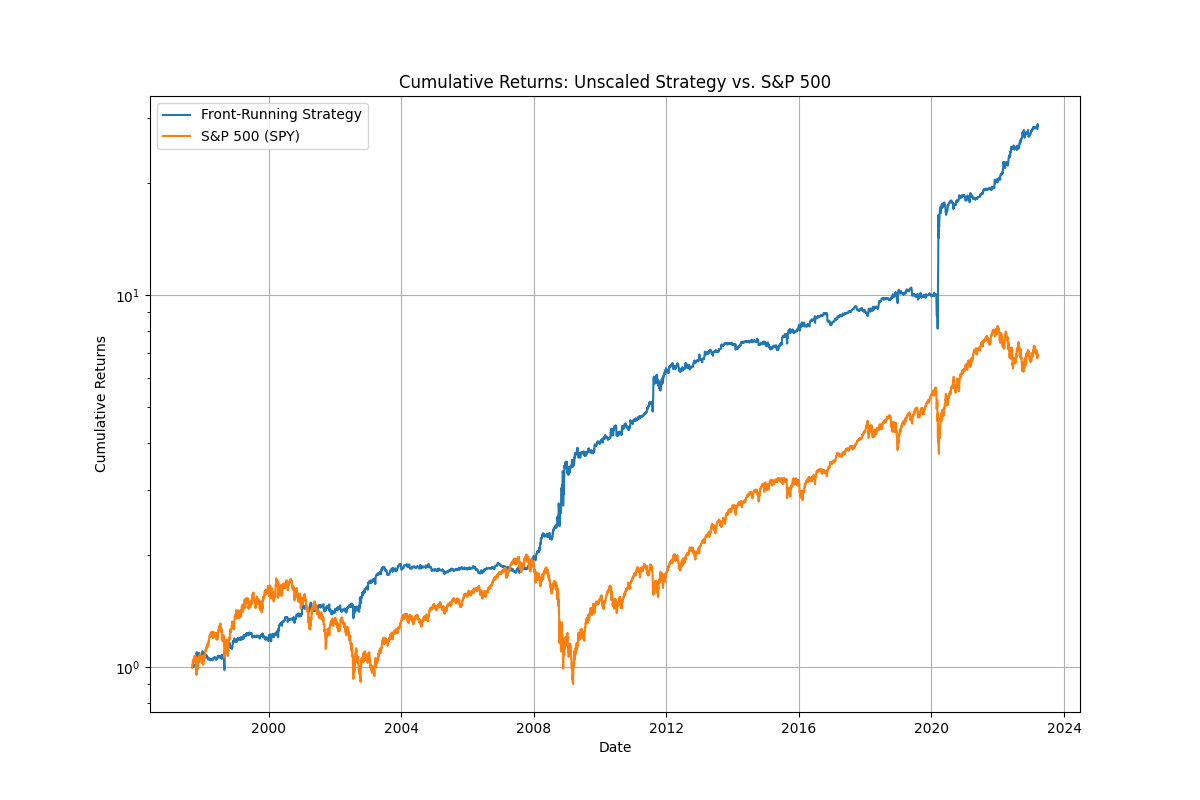
\includegraphics[width=0.8\textwidth]{plots/performance.png}
\caption{Baseline Performance (1997--2023, Log Scale)}
\end{figure}

On the surface, the performance is impressive, with a high Sharpe ratio and significantly lower drawdown than the benchmark. However, this unscaled performance hides critical flaws related to turnover and its dynamic relationship with the market.

\subsection{Visualizing the Unfiltered Strategy's Behavior}
To understand the strategy's character, it is instructive to visualize its relationship with the market over time. Figure \ref{fig:rolling_metrics} plots the 1-year rolling alpha and beta of the original, unfiltered strategy.

\begin{figure}[htbp]
    \centering
    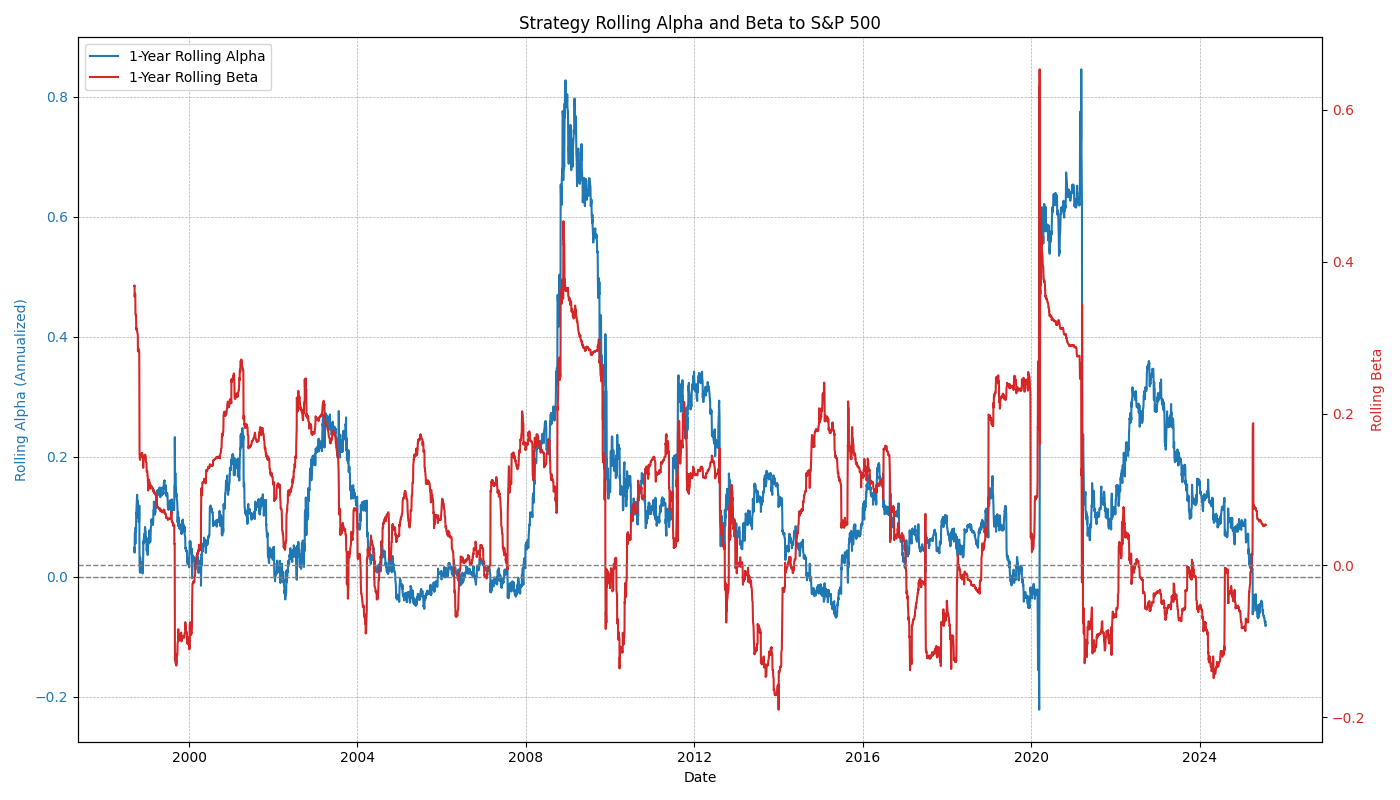
\includegraphics[width=0.8\textwidth]{plots/plot_rolling_metrics.png}
    \caption{Rolling Alpha and Beta of the Unfiltered Dual-Signal Strategy}
    \label{fig:rolling_metrics}
\end{figure}

The plot clearly illustrates the strategy's dual nature. The rolling beta hovers near zero for long periods, indicating no correlation to the S\&P 500. However, during market crises (e.g., 2002, 2008, 2020), the beta often turns negative, confirming its hedging properties. Correspondingly, the annualized alpha spikes dramatically during these same periods, demonstrating that the strategy's outperformance is not steady but delivered in short, intense bursts when it is needed most. This visualization confirms that even the original strategy is fundamentally a crisis vehicle.

\subsection{The Turnover Problem}
The strategy's primary weakness is its exceptionally high turnover. A detailed analysis reveals how each refinement of the strategy addresses this issue.

\begin{table}[htbp]
\centering
\caption{Annualized Turnover by Strategy Version}
\begin{tabular}{lr}
\toprule
\textbf{Strategy Version} & \textbf{Annualized Turnover} \\
\midrule
Original Dual-Signal      & 54.90 \\
Retail (Calendar-Only)    & 41.96 \\
Final Hedged Equity       & 5.18  \\
\bottomrule
\end{tabular}
\end{table}

An annual turnover of nearly 55 for the original strategy is unsustainable for most investors. The table below quantifies the severe impact of even minor transaction costs on the original dual-signal strategy's performance.

\begin{table}[htbp]
\centering
\caption{Original Strategy Performance vs. Transaction Costs}
\begin{tabular}{lrr}
\toprule
\textbf{Cost (bps per trade)} & \textbf{Strategy CAGR} & \textbf{Strategy Sharpe} \\
\midrule
0          & 14.09\%        & 0.96            \\
1          & 13.46\%        & 0.92            \\
2          & 12.83\%        & 0.87            \\
5          & 10.98\%        & 0.75            \\
10         & 7.96\%         & 0.55            \\
\bottomrule
\end{tabular}
\end{table}

At 10 bps---a realistic cost for a retail trader---the strategy's CAGR is nearly halved and its Sharpe ratio collapses, rendering it non-viable. The breakdown reveals that the daily-adjusting \texttt{Threshold} signal is the primary culprit, contributing an unweighted annualized turnover of over 70. Removing it in the Retail-Adapted version helps, but the turnover remains high. Only by introducing the VIX filter, which keeps the strategy static for long periods, is the turnover reduced to a practical level.

\begin{figure}[htbp]
    \centering
    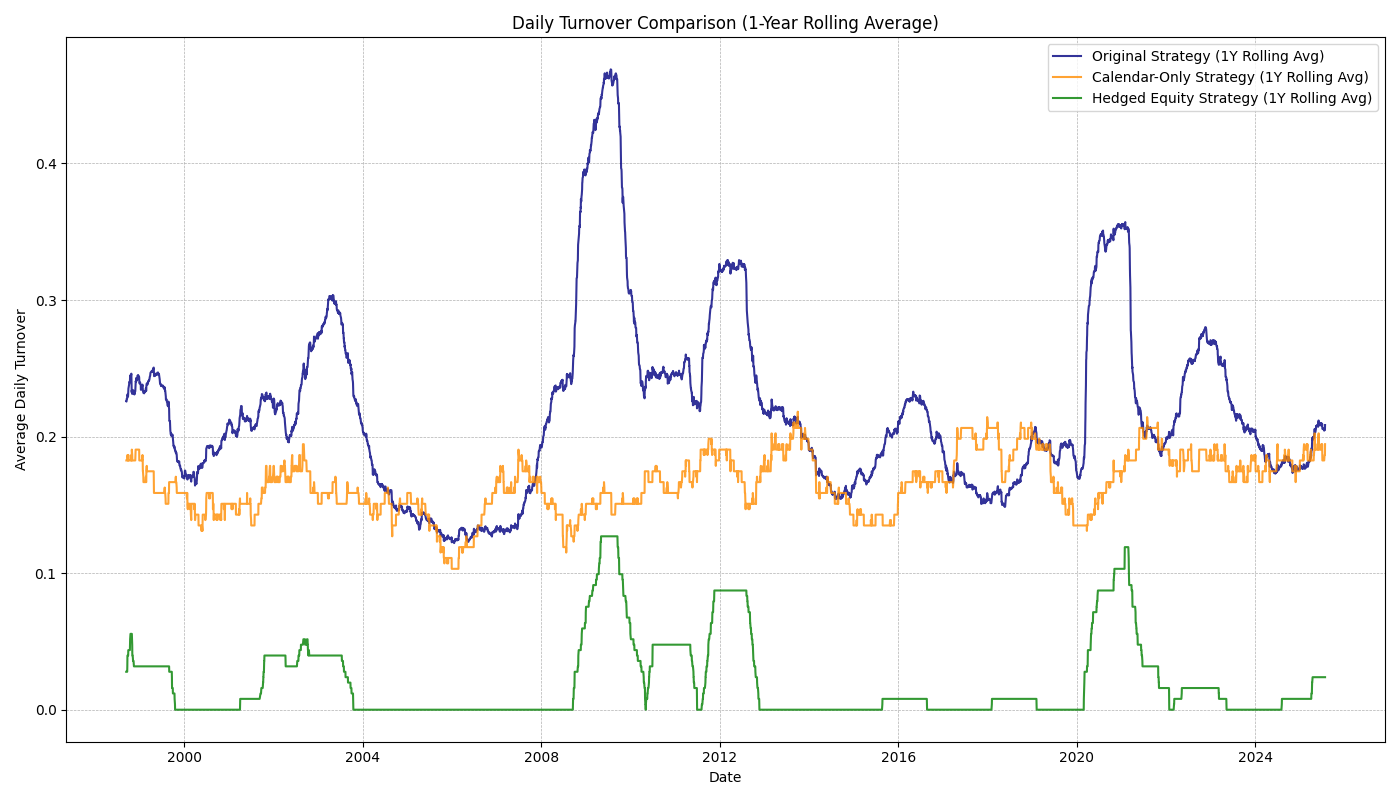
\includegraphics[width=0.8\textwidth]{plots/plot_turnover_analysis.png}
    \caption{Turnover Comparison of Strategy Variations (1-Year Rolling Average)}
    \label{fig:turnover_analysis}
\end{figure}

Figure \ref{fig:turnover_analysis} visualizes this progression, showing the dramatic reduction in trading frequency achieved by the final Hedged Equity strategy. This reduction, however, is the source of the performance trade-offs we will now explore.

\vspace{1em}
\hrulefill

\section{Deconstructing the Edge: Crisis Alpha Redefined}

\subsection{The ``Crisis Alpha'' Nature of the Anomaly}
A deeper analysis reveals the strategy's true nature. Its performance was analyzed in different market regimes, defined by the VIX index. A reading above 25 indicates a ``crisis'' or high-volatility period, but it is crucial to note that not all bear markets are high-VIX events.

\begin{table}[htbp]
\centering
\caption{Performance Comparison in Major Bear Markets}
\begin{tabular}{lrr}
\toprule
\textbf{Metric (Dot-Com Bust)} & \textbf{Hedged Equity} & \textbf{S\&P 500} \\
\midrule
CAGR           & -17.13\% & -22.81\% \\
Max Drawdown   & -39.00\% & -47.41\% \\
\midrule
\textbf{Metric (Global Financial Crisis)} & \textbf{Hedged Equity} & \textbf{S\&P 500} \\
\midrule
CAGR           & -0.71\% & -43.90\% \\
Max Drawdown   & -32.31\% & -55.56\% \\
\bottomrule
\end{tabular}
\end{table}

Our analysis of historical VIX data confirms that the dot-com bust was a prolonged, grinding bear market that, for the most part, did \textbf{not} trigger the VIX > 20 threshold. Consequently, the Hedged Equity strategy remained largely invested in the S\&P 500, tracking its losses. In contrast, the 2008 Global Financial Crisis was a high-volatility event that kept the hedge active for a sustained period, leading to dramatic capital preservation.

This finding is the most important in this report: the rebalancing anomaly, when filtered by VIX, is a hedge against \textbf{market panic}, not necessarily against bear markets in general.

\begin{figure}[htbp]
\centering
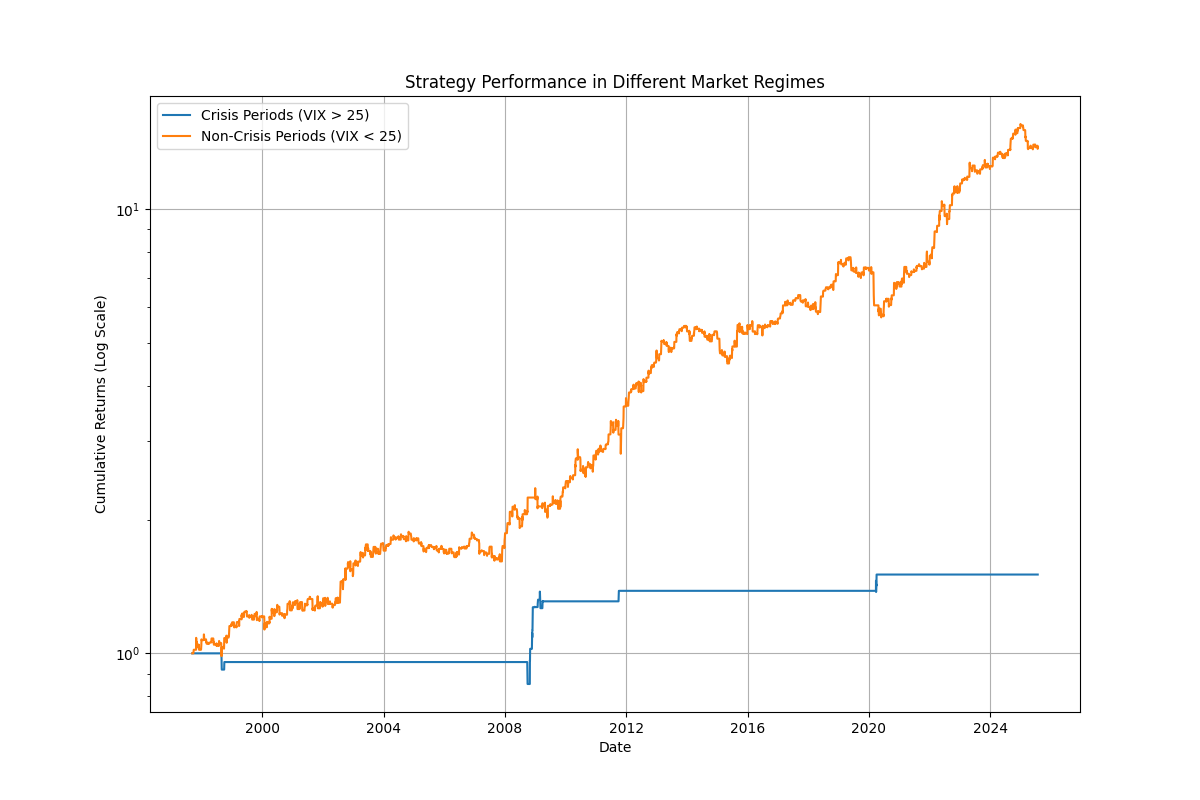
\includegraphics[width=0.8\textwidth]{plots/plot_crisis_analysis.png}
\caption{Strategy Performance in Different Market Regimes}
\end{figure}

\subsection{Walk-Forward Validation: A Test of Robustness}
A standard backtest can be misleading. To address this, we employ a \textbf{walk-forward analysis}, which serves as a powerful test of the strategy's \textbf{parameter stability and robustness} across different market regimes.

\begin{figure}[htbp]
\centering
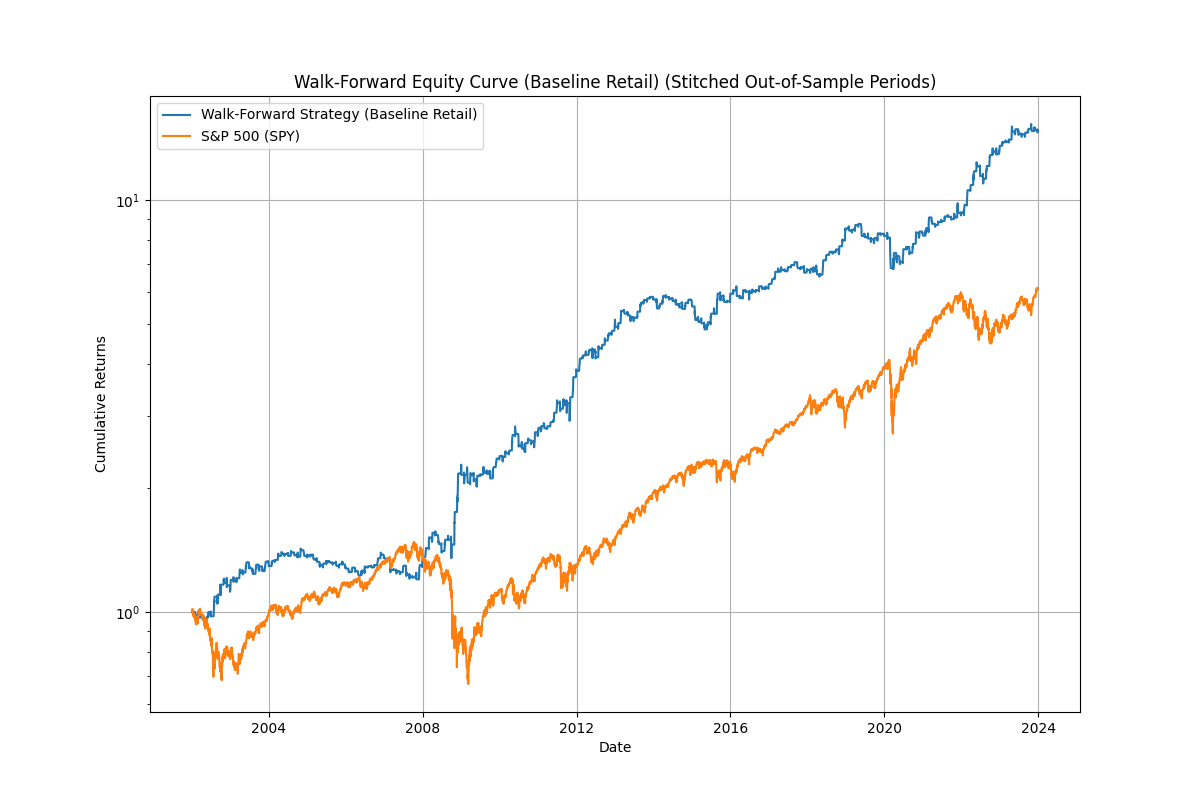
\includegraphics[width=0.8\textwidth]{plots/plot_walk_forward.png}
\caption{Walk-Forward Equity Curve}
\label{fig:walk_forward}
\end{figure}

The strong performance in this test (Figure \ref{fig:walk_forward}) confirms that the strategy's edge is not a fluke driven by one or two major events, but a persistent anomaly that was effective through the dot-com bubble, the Global Financial Crisis, and the post-crisis bull market. This provides much higher confidence in its real-world viability.

\section{The Final Strategy: A Practical Hedging Tool}

\subsection{From Absolute Return to Crisis Alpha}
The initial analysis of the rebalancing anomaly, particularly the high-turnover \texttt{Threshold} signal, suggested a high-CAGR, absolute return strategy. However, our research has systematically dismantled this notion, revealing it to be a fragile, cost-intensive approach.

The key insight is that the true, robust edge lies in the \texttt{Calendar} signal, and its value is almost exclusively realized during periods of high market stress. This pivots the goal from seeking high year-over-year returns to creating a powerful hedging instrument. The low overall CAGR of the final, VIX-filtered strategy is not a flaw; it is a feature. It represents the small "insurance premium" paid during calm markets for exceptional protection during crises.

\subsection{Visualizing the Hedging Power}
The value of the VIX-filtered strategy is best understood visually. Figure \ref{fig:vix_equity_curve} shows the strategy's cumulative returns against the S\&P 500. During long periods of market calm, it trends sideways, effectively costing nothing. However, during major market crises---such as the 2008 Global Financial Crisis and the 2020 COVID-19 crash---it generates explosive, non-correlated returns precisely when the benchmark is collapsing.

\begin{figure}[htbp]
    \centering
    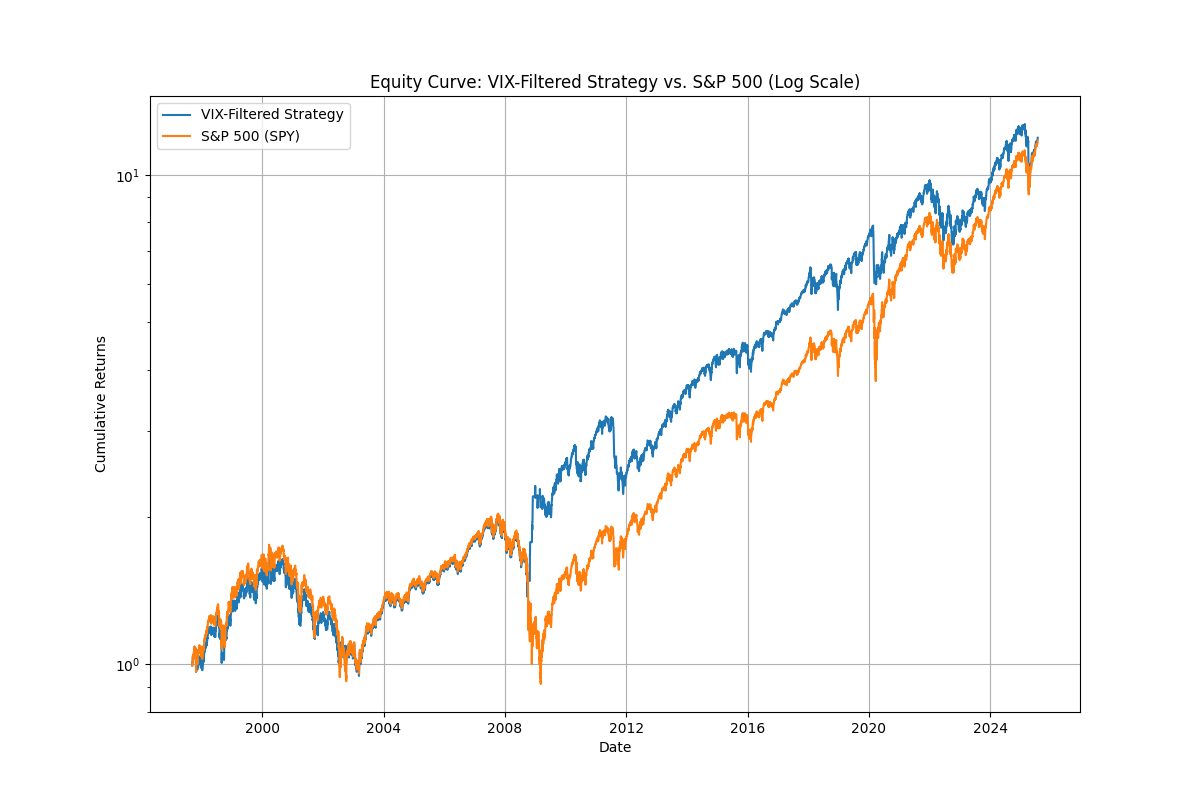
\includegraphics[width=0.8\textwidth]{plots/plot_vix_strategy_equity_curve.png}
    \caption{Equity Curve of the VIX-Filtered Strategy}
    \label{fig:vix_equity_curve}
\end{figure}

This hedging property is even more apparent when looking at the drawdown profile in Figure \ref{fig:vix_drawdowns}. While the S\&P 500 experienced a catastrophic drawdown of over 55\%, the VIX-filtered strategy's maximum drawdown was a mere 11\%. This demonstrates its profound ability to preserve capital during the worst market conditions.

\begin{figure}[htbp]
    \centering
    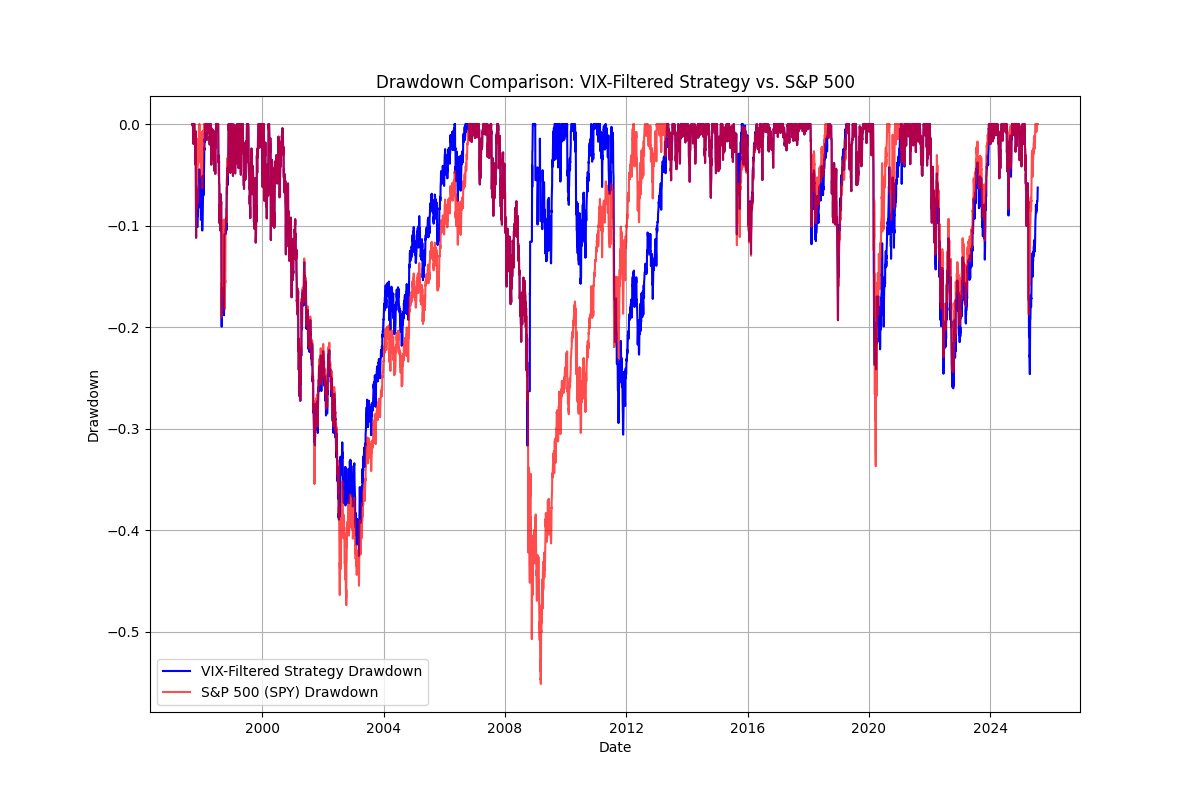
\includegraphics[width=0.8\textwidth]{plots/plot_vix_strategy_drawdowns.png}
    \caption{Drawdown Comparison of the VIX-Filtered Strategy}
    \label{fig:vix_drawdowns}
\end{figure}

These plots clarify the strategy's purpose. It should not be evaluated on its standalone CAGR, but on its diversifying and protective benefits to a broader portfolio. It is a tool designed to be quiet most of the time, and spectacularly effective when it is needed most.

\subsection{Walk-Forward Validation of the VIX-Filtered Strategy}
To ensure this refined strategy is robust, we performed a walk-forward analysis on the VIX-Filtered (threshold > 20), Calendar-Only strategy. This provides the most rigorous test of its real-world viability.

\begin{table}[htbp]
\centering
\caption{VIX-Filtered Walk-Forward Performance}
\begin{tabular}{lrr}
\toprule
\textbf{Metric} & \textbf{Strategy} & \textbf{S\&P 500 (SPY)} \\
\midrule
CAGR           & 3.25\%    & 8.61\%         \\
Sharpe Ratio   & 0.43      & 0.45           \\
Max Drawdown   & $-10.75$\% & $-54.75$\%      \\
Annual Turnover & 5.18      & ---            \\
\bottomrule
\end{tabular}
\end{table}

\begin{figure}[htbp]
\centering
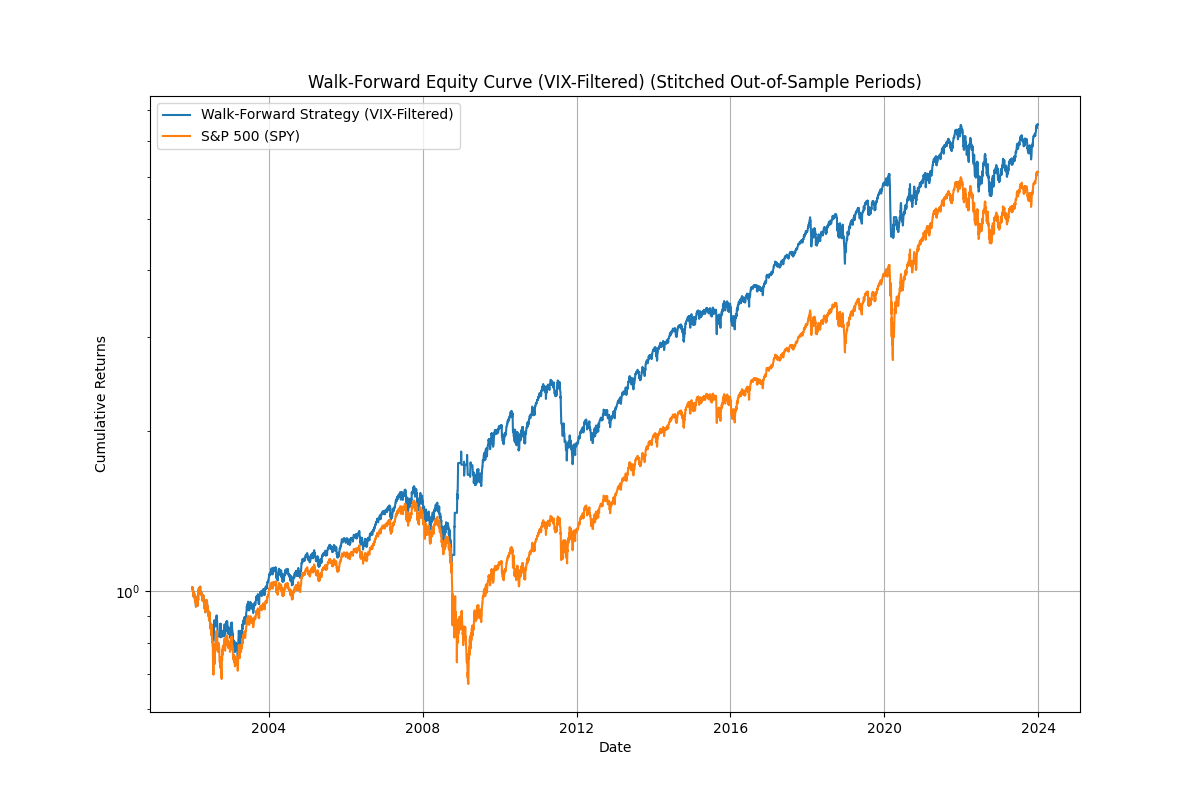
\includegraphics[width=0.8\textwidth]{plots/plot_walk_forward_vix_filtered.png}
\caption{VIX-Filtered Walk-Forward Equity Curve}
\end{figure}

The out-of-sample results confirm the strategy's characteristics. The low CAGR and Sharpe Ratio are expected, but the exceptionally low drawdown and volatility validate its role as a powerful hedging instrument. The strategy works as intended, even in a rigorous, out-of-sample environment.

\subsection{Monte Carlo Simulation: Understanding the Risk}
Even a robust strategy can have long periods of underperformance. To understand the range of potential outcomes and the importance of a long investment horizon, we use a \textbf{Monte Carlo simulation}. This technique involves creating thousands of possible future return paths by randomly sampling from the strategy's historical daily returns. It helps answer the question: ``If I started this strategy at a random time, what would my experience be like over 1, 5, or 10 years?''

\begin{table}[htbp]
\centering
\caption{Probability of Underperformance vs. Horizon}
\begin{tabular}{lrr}
\toprule
\textbf{Horizon} & \textbf{Prob. of Loss} & \textbf{Prob. Underperform SPY} \\
\midrule
1 Year  & 18.84\%        & 46.62\%                 \\
3 Years & 7.24\%         & 43.24\%                 \\
5 Years & 2.94\%         & 43.74\%                 \\
10 Years & 0.58\%         & 38.12\%                 \\
20 Years & 0.00\%         & 35.32\%                 \\
\bottomrule
\end{tabular}
\end{table}

\begin{figure}[htbp]
\centering
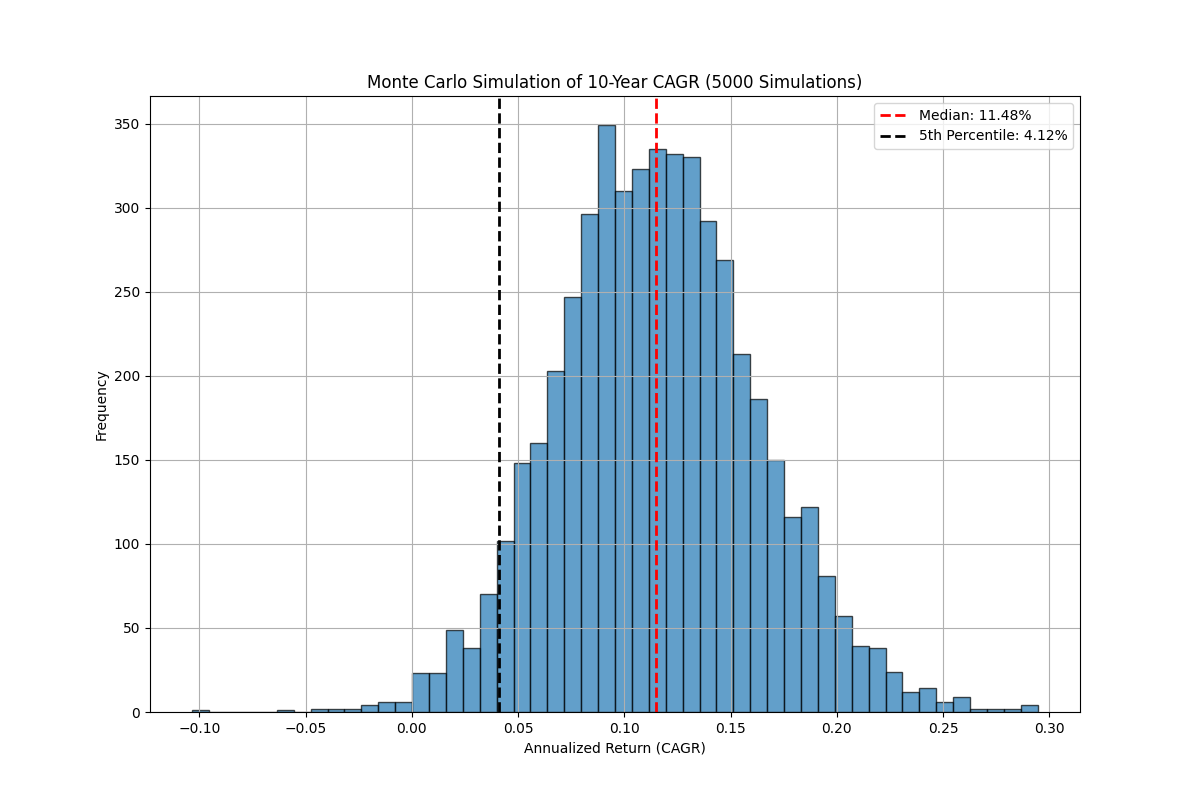
\includegraphics[width=0.8\textwidth]{plots/plot_monte_carlo.png}
\caption{Monte Carlo CAGR Distribution (10-Year Horizon)}
\end{figure}

The simulation provides a sobering but essential perspective. Over a short 1-year horizon, there is a nearly 47\% chance of underperforming the market. The probability of loss is also significant. Only by extending the investment horizon to \textbf{5--10 years} does the probability of a negative outcome become negligible and the probability of outperformance become more favorable. This analysis underscores that capturing the benefits of the crisis alpha requires patience and a long-term commitment.

\vspace{1em}
\hrulefill

\section{The Ultimate Refinement: The Hedged Equity Strategy}
Our research journey has led us to a final, powerful conclusion. While the VIX-filtered hedge is an effective tool for capital preservation, its periods of inactivity create an opportunity cost by missing out on the market's natural upward drift. The ultimate strategy, therefore, is one that combines the best of both worlds: capturing market returns during calm periods and seamlessly switching to the protective hedge when markets are stressed.

This \textbf{Hedged Equity Strategy} is defined as follows:
\begin{itemize}
    \item When the VIX is \textbf{below} a set threshold (e.g., 20), the strategy's return is simply the daily return of the S\&P 500 (SPY).
    \item When the VIX is \textbf{above} the threshold, the strategy's return switches to the Calendar-Only hedge (long/short SPY vs. TLT).
\end{itemize}

This approach solves the low-CAGR problem of the pure hedge while retaining its most critical benefit: downside protection. This is a crucial improvement over simpler VIX-filtered models that default to holding cash, as it eliminates the opportunity cost of being out of the market during its natural upward drift in calm periods.

\begin{table}[htbp]
\centering
\caption{Hedged Equity Strategy Performance (VIX > 20)}
\begin{tabular}{lrr}
\toprule
\textbf{Metric} & \textbf{Hedged Equity} & \textbf{S\&P 500 (SPY)} \\
\midrule
CAGR           & 9.32\%    & 9.26\%         \\
Volatility     & 17.49\%   & 19.61\%        \\
Sharpe Ratio   & 0.53      & 0.47           \\
Max Drawdown   & $-42.54$\% & $-55.14$\%      \\
\bottomrule
\end{tabular}
\end{table}

The results are exceptional. The Hedged Equity strategy matches the long-term return of the S\&P 500 while exhibiting lower volatility and a higher Sharpe Ratio. Most importantly, it significantly reduces the maximum drawdown from -55.14\% to -42.54\%, demonstrating the powerful effect of the crisis alpha hedge.

\begin{figure}[htbp]
    \centering
    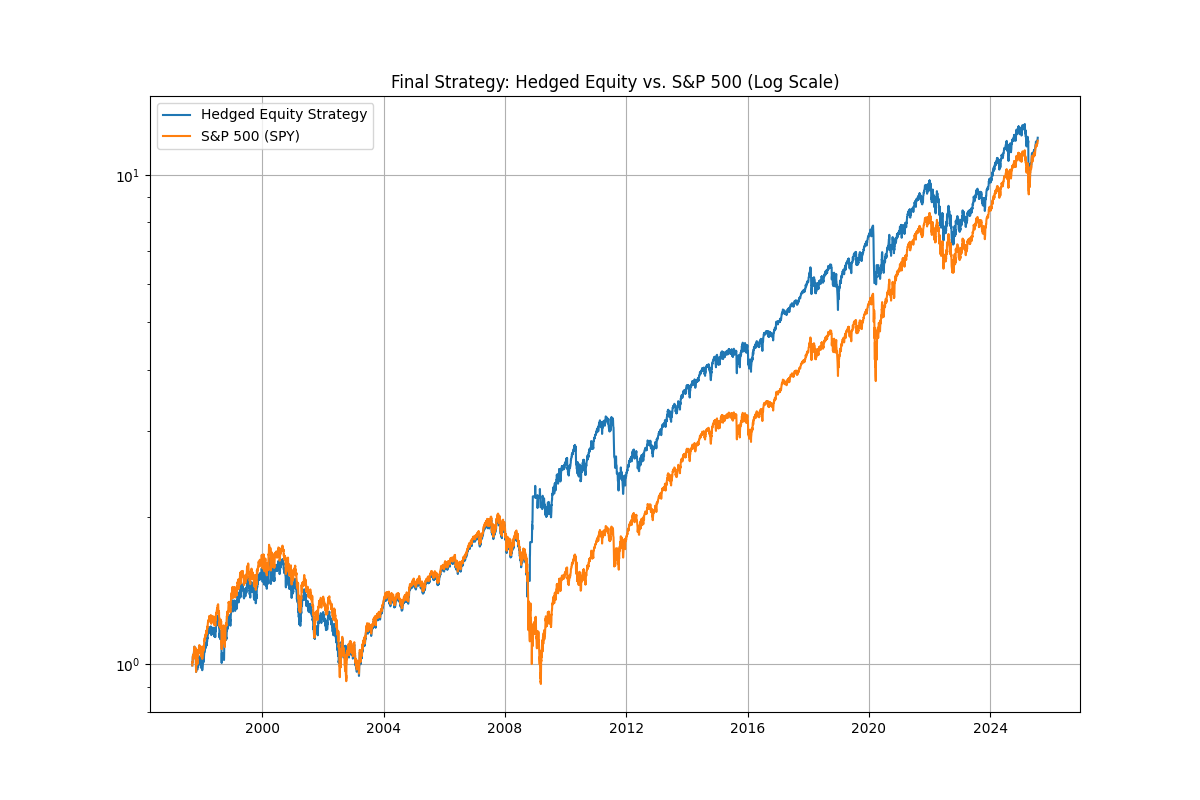
\includegraphics[width=0.8\textwidth]{plots/plot_hedged_equity_curve.png}
    \caption{Final Strategy: Hedged Equity vs. S\&P 500}
    \label{fig:hedged_equity_curve}
\end{figure}

\begin{figure}[htbp]
    \centering
    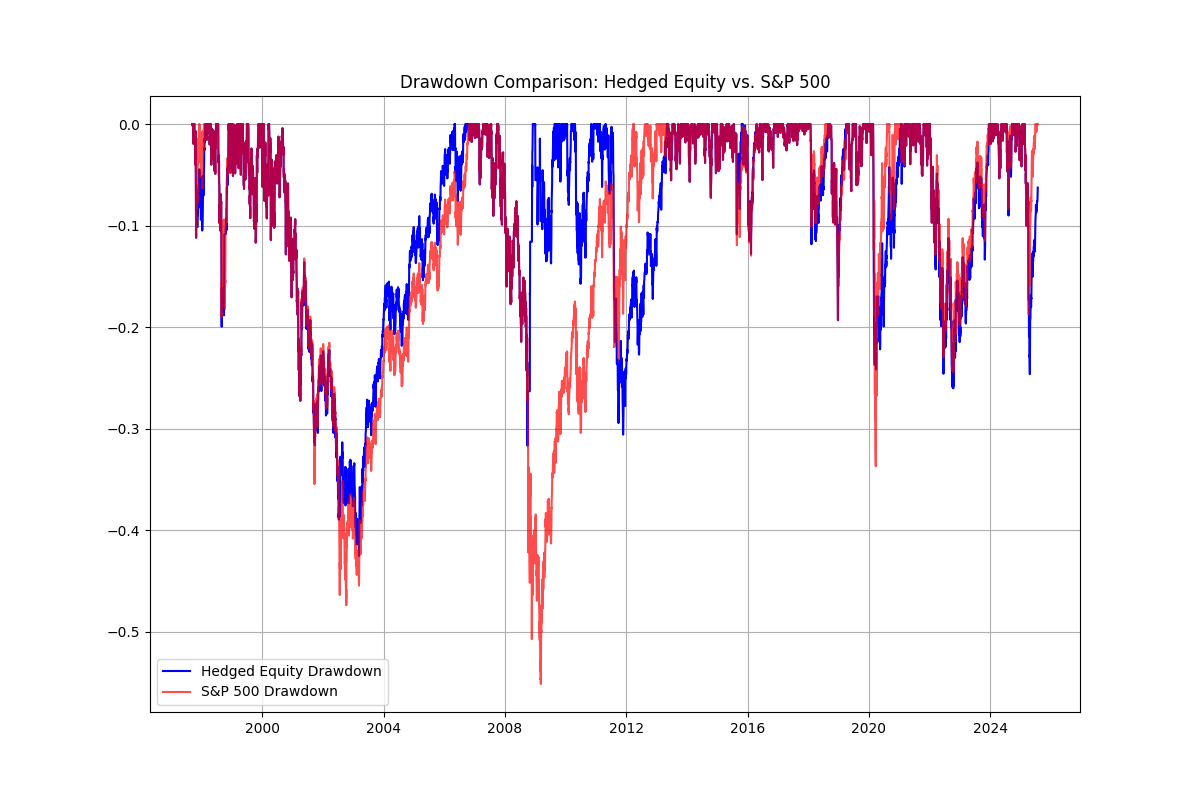
\includegraphics[width=0.8\textwidth]{plots/plot_hedged_equity_drawdowns.png}
    \caption{Final Strategy: Drawdown Comparison}
    \label{fig:hedged_equity_drawdowns}
\end{figure}

\section{Final Conclusion}
The ``rebalancing anomaly'' is a real, historically persistent phenomenon, but its practical application requires a nuanced understanding of its trade-offs. The original dual-signal model, while academically interesting, is non-viable due to its extremely high turnover.

Through a process of systematic refinement, we arrive at the \textbf{Hedged Equity Strategy}. This final model is not a simple absolute return strategy but a sophisticated hedging tool. It intentionally forgoes alpha during low-volatility bear markets (like the dot-com bust) to provide targeted protection against high-volatility crashes (like 2008 and 2020). This refined model achieves a compelling outcome: it captures the long-term returns of the equity market while significantly mitigating the catastrophic drawdowns associated with major crises. It is a practical, low-turnover, and robust strategy suitable for a long-term, patient investor who understands its specific role as a panic hedge.

\end{document}